\chapter{Implementacja}
\label{cha:implementacja}

\section{Przygotowanie danych}
\label{cha:przygotowanie}

Przygotowany został moduł \textit{data}, w którym dane są wczytywane i poddawane obróbce koniecznej do przeprowadzenia prawidłowego procesu uczenia. 

Każde słowo ze zbioru danych zapisano do słownika \textit{word2idx} i przypisano mu unikalny indeks. W celu przyspieszenia działania programu zamieniono wszystkie słowa w zdaniach na ich indeksy ze słownika. 

Lista etykiet określających rodziców została zastąpiona słownikiem, w którym kluczami są kolejne węzły, a wartościami \textendash \ lista ich dzieci lub pusta lista w przypadku braku dzieci. 

\section{Implementacja modelu}
\label{cha:implementacjamodelu}

Mamy trzy sekwencje, po których potrzebujemy przeiterować w tym samym czasie: listę słów, która zawierającą indeksy ze słownika \textit{word2idx}, listę dzieci poszczególnych węzłów oraz listę etykiet ich wydźwięku. Potrzebna jest zatem pętla, która przejdzie przez te sekwencje. Nie znane są jednak na tym etapie wartości tych zmiennych, ani nawet ich długości, nie można więc użyć zwykłej pętli \textit{while}. Wykorzystano w tym przypadku \textit{tf.while\_loop} z biblioteki TensorFlow (listing 1), która powtarza funkcję \textit{pętla} dopóki \textit{warunek} jest prawdziwy. 

\begin{listing}[]
\lstinputlisting[language=python]{listing/while.py}
\caption{Pętla generująca tablicę wyjść.}
\end{listing}

Warunkiem zakończenia pętli jest tutaj koniec zdania, natomiast ciało wykonywanej funkcji przedstawia listing 2. Dla każdego dziecka danego węzła obliczane są wartości poszczególnych bramek LSTM według wzorów podanych w rozdziale czwartym. W momencie gdy algorytm dojdzie do korzenia drzewa, który znajduje się na końcu listy, przeprowadzane jest mapowanie słowa na wektor liczb rzeczywistych. 
\\

\begin{listing}[]
\begin{algorithmic}
\FOR{dziecko \textbf{in} lista dzieci} 
\IF {węzeł nie jest korzeniem} 
        \STATE $h_1 = oblicz\_bramki(h_1, wyjscie(dziecko))$
\ELSE
        \STATE $h_1 = mapuj(aktualne\ slowo)$
        \ENDIF
\ENDFOR
\end{algorithmic}
\caption{Funkcja wyznaczająca stan aktualnego węzła.}
\end{listing}

Po zakończeniu pętli otrzymujemy ostateczną wyjściową tablicę. Mnożona jest ona przez wyjściową macierz wag i wyjściowy bias. Otrzymany wynik wykorzystywany jest do wyznaczenia wartości funkcji kosztu. W programie użyta została funkcja \textit{sparse\_softmax\_cross\_entropy\_with\_logits}, którą stosuje się do problemów klasyfikacji wieloklasowej. 

Zasadniczo cała implementacja sprowadza się do następujących etapów:
\begin{itemize}
  \item Wczytanie danych
  \item Zbudowanie modelu LSTM
  \item Wyznaczenie wartości kosztu
  \item Uruchomienie pętli uczenia
  \item Wyświetlenie wyników
 \end{itemize}


\section{Dobór parametrów}
\label{cha:parametry}

\subsection{Wybór optymalizatora}
Optymalizator to algorytm mający na celu znalezienie minimum zadanej funkcji kosztu. Wybór metody optymalizacji używanej w procesie uczenia miał duży wpływ na otrzymywane wyniki, co widać w tabeli 6.1. Zbadano optymalizator gradientu prostego, a także jego modyfikacje: \textit{Momentum}, \textit{Adagrad} oraz \textit{Adam}. Powodem wybrania tych czterech algorytmów do analizy był fakt, że powtarzały się one najczęściej w znalezionych przykładach implementacji róznych modeli LSTM. 

W każdym przypadku rozmiar partii wynosił 32, natomiast wartość wskaźnika uczenia \textendash \ 0.01. W tabeli 6.1 widać bardzo dużą różnicę między wynikami osiąganymi przez optymalizator Adam, a pozostałymi algorytmami. Nie ma więc wątpliwości, że Adam najlepiej sprawdzi się w trenowaniu zaporojektowanej tutaj sieci.

\begin{table}[H]
\centering
\begin{tabular}{|l|c|c|c|c|}
\hline
\textbf{Klasyfikator}           & Adam             & Adagrad         & Gradient prosty              & Momentum         \\ \hline
\textbf{Dokładność uczenia}     & \textbf{96,78\%} & 77,3\% & 89,47\% & 86,59\% \\ \hline
\textbf{Wartość funkcji kosztu} & \textbf{2.56}           & 11,12         & 5,2            & 4,58           \\ \hline
\end{tabular}%

\caption{Porównanie wyników po 10 epokach uczenia.}
\label{table:bf-sa}
\end{table}

\subsection{Wskaźnik uczenia}

Wskaźnik uczenia (\textit{ang. learning rate}) wpływa na to, jak szybko aktualizowane są wagi \textendash \ zbyt wysoka wartość sprawia, że sieć może przeskakiwać minima, natomiast zbyt niska znacznie wydłuża czas uczenia. Tabela 6.2 przedstawia porównanie wyników dla 32-wymiarowej warstwy ukrytej i optymalizatora Adam. Jak widać, wysoki wskaźnik uczenia się nie sprawdza. W bibliotece TensorFlow dla optymalizatora Adam domyślnym wskaźnikiem uczenia jest wartość 0,001, jednak w opisywanym tutaj przypadku lepiej sprawdza się wartość 0,01, gdyż osiąga dobre wyniki w rozsądnym czasie. 

\begin{table}[H]
\centering

\begin{tabular}{|l|c|c|c|}
\hline
\textbf{Wskaźnik uczenia}       & 0,1     & 0,01    & 0,001   \\ \hline
\textbf{Dokładność uczenia}     & 77,25\% & \textbf{96,78\%} & 96,64\% \\ \hline
\textbf{Wartość funkcji kosztu} & 12.05 & \textbf{2.56}  & 4.31  \\ \hline
\end{tabular}%

\caption{Porównanie wyników po 10 epokach uczenia.}
\label{table:bf-sa}
\end{table}

\subsection{Wymiary warstwy ukrytej}

Działanie modelu zostało sprawdzone dla różnych wymiarów warstwy ukrytej. W każdym przypadku użyty został optymalizator Adam, natomiast wskaźnik uczenia wynosił 0.01. Jak widać w tabeli 6.2, wartości w zakresie 8-32 dają bardzo zbliżone wyniki w kwestii dokładności uczenia i wartości funkcji kosztu, z niewielką przewagą 32-wymiarowej warstwy ukrytej.

W literaturze nie znaleziono uzasadnienia wpływu tego parametru na ostateczne wyniki, można więc uznać dobór wymiarów warstwy ukrytej za kwestię indywidualną. Im większa jest ta wartość, tym dłuższy jest czas obliczeń: przy 16 wymiarach czas obliczeń jednej epoki wynosił 150 s, przy 32 \textendash \ 200 s, natomiast dla 64-wymiarowego stanu ukrytego już 337 s.
\begin{table}[H]
\centering
\begin{tabular}{|l|c|c|c|c|l|}
\hline
\textbf{Wymiary warstwy ukrytej}         & 4       & 8       & 16      & 32      & 64  \\ \hline
\textbf{Dokładność uczenia}     & 95,46\% & 97,02\% & 96,93\% & \textbf{97,09\%} & 96,44\% \\ \hline
\textbf{Wartość funkcji kosztu} & 3.55  & 2.39  & 2.3   & \textbf{2.25}  & 2.55\% \\ \hline
\end{tabular}%

\caption{Porównanie wyników po 15 epokach uczenia.}
\label{table:bf-sa}
\end{table}

\section{Regularyzacja modelu}


\label{cha:regulacja}
\subsection{Regularyzacja funkcji kosztu}
W celu zwiększenia wydajności modelu i uniknięcia przeuczenia (nadmiernego dopasowania) stosuje się różne techinki regularyzacji. Jedną z typowych metod jest regularyzacja l2, która polega na wyznaczeniu regularyzacyjnej funkcji kosztu będącej sumą normy $L^2$ obliczonej dla wag wejściowych \textit{$W_{xi}$} oraz dla wag wyjściowych \textit{U}, co przedstawia wzór 6.1. Wartość 0,02 jest tu dobranym parametrem optymalnym do używanego modelu. Wyznaczenie całkowitego kosztu polega na zsumowaniu wartości funkcji kosztu i wartości funkcji regularyzacji.

\begin{equation}
r = 0,02 * L^2(W_{xi}) + L^2(U) \end{equation}

\subsection{Wpływ wag na proces uczenia}
Samo zaincjalizowanie macierzy wag losowymi wartościami może doprowadzić do problemu znikającego lub eksplodującego gradientu, który został opisany w rozdziale 4. Aby temu zapobiec, wartości początkowe macierzy wyznaczono za pomocą heurystyki ze wzoru 6.1.
\begin{equation}
W = random(M, N) * \sqrt{\frac{1}{M+N}}
\end{equation}


\label{sec:etykiety}
\begin{figure}[H]
    \centering
    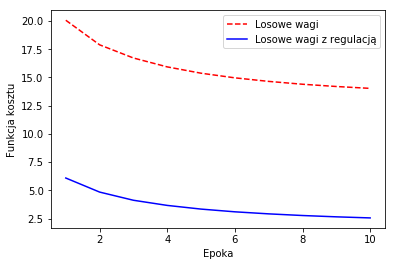
\includegraphics[clip]{weight_regulation.png}
    \caption{Porównanie wyników dla macierzy wag inicjalizowanych losowo oraz losowo z regularyzacją.}
\end{figure}
Na wykresie 6.1 widać jak dużą wpływ na osiąganą wartość funkcji kosztu ma zastosowanie powyższej regularyzacji.

Ciekawym eksperymentem okazało się również zmniejszenie wag poprzez pomnożenie każdej macierzy przez parametr o wartości 0,05. Jak widać na wykresie 6.2, nie wprowadza to znacznych zmian, choć to ulepszenie pozwala na osiągnięcie danej wartości funkcji kosztu o dwie epoki szybciej niż w przypadku, gdy nie mnożymy macierzy przez parametr. 

\label{sec:etykiety}
\begin{figure}[H]
    \centering
    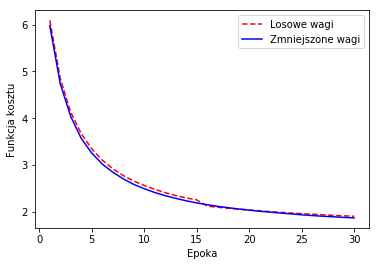
\includegraphics[clip]{min_weights.png}
    \caption{Porównanie wyników dla macierzy wag inicjalizowanych losowo oraz losowo ze zmniejszonymi wagami.}
\end{figure}


